\label{arduino}
%The Indirect methods consist of estimating the energy base how much time he spent in which state and how much the seeks, reads, and writes, and knowing much which operation costs and how much energy he spent every time he which is every state. With that knowledge, we can estimate how much energy consumption during that time. This approach produces good results, but since all energy is an estimate, this procedure including an error margin on the results.

%The other approach is the direct method by using external hardware, this method consists of measuring Electric Potential Difference on the disk. This method is a lot precise since the results are real, but the downsize it is that have an impact on the overall performance, this impact it only notices on a big scale~\cite{portela2016}.

Here it will show why Arduino was chosen to measure energy consumption on disk storage, which method he uses, and how he works.

In this case, for measured disk consumption we opt for an instant power measurement approach made by \citeauthor{portela2016} instead of a Model Estimation. An Instant power measurement approach is a reliable choice because it is one of the simple solutions to achieve the objectives intended, and it is low-cost. Here we want to ensure that our results are precise and reliable, and since our measurements are on a small scale, it doesn't have an impact on the overall system. This solution provides what is needed without significant drawbacks ~\cite{portela2016}.


Since it is necessary for data storage and handling of energy consumption, a mere ammeter won't do the work here. Thus to gather the measurements it was chosen an Arduino Uno with a current sensory. Figure \ref{fig:satacable} presents the scheme of an Arduino UNO with a current sensory connected to a \gls{sata} cable. The \gls{sata} cable is responsible for distributing energy to the disk and data exchange between the secondary storage and the computer.  So to get the energy consumption on the disk, the current sensor must be connected to the \gls{sata} cable that is responsible for distributing energy ~\cite{portela2016}.

\begin{figure}[H]
  \centering
  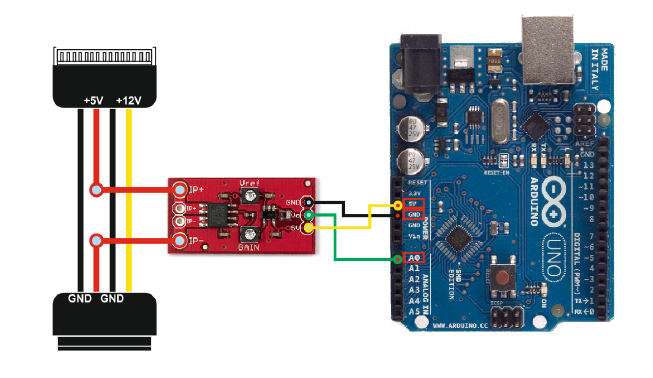
\includegraphics[width=0.8\columnwidth]{Chapters/images/arduino.png}  \caption{Scheme of connections between \gls{sata} cable, current sensor and Arduino used to measurement secondary storage.}
  \label{fig:satacable}
\end{figure}



The current sensor used was the Low Current Sensor Breakout. This current sensor is made by SparkFun and can measure the current regardless of whether the signal is continuous or alternating.  This sensor has an operational amplifier phase to control the gain, which can measure lower currents more precisely ~\cite{portela2016}.

Furthermore, Arduino UNO must be able to read the analog voltage presented by the sensor and communicate these values to the computer connected to it through the serial port. For this, a program was made that would get take constant readings at the analog voltage and send them every 0.1 seconds. An example of this code is on the Listing \ref{lst:arduinocode} where the reading is made every millisecond and then is made the average of the last one hundred milliseconds, which send this information to the computer system connected to the Arduino.

  \begin{lstlisting}[ caption={ Arduino source code for reading the analog signal from the current sensor},label={lst:arduinocode},language=C,
    basicstyle=\small
]
void loop() {
  /* Initialization */
  float average_a0 = 0; // Raw reading from pin
  float voltage = 0; // Voltage in V
  float current = 0; // Current in A
  float wattage = 0; // Wattage in W
  float power = 0; // Power in J
  /* Average loop */
  for(int i = 0; i < n_reads ; i++) {
    average_a0 += analogRead(sensorPin_0);
    delay(loop_delay);  }
  /* Formula based computations */
  average_a0 /= n_reads;
  voltage = (average_a0 / 1024.0) * 5;
  current = current_eq(voltage);
  wattage = voltage * current;
  power = wattage * interval;
  Serial.println(power, 3);
  Serial.flush();}

\end{lstlisting}



